\section{Smooth conductors: the sphere and the torus}
\label{sec:smooth}

\subsection{The sphere}

We begin with the familiar domain of the unit sphere, for which the Mie series provides the exact scattered field. The polarisation vector is $\bp = (0,1,0)^\top$ and the propagation direction is $\bd = (0,0,-1)^\top$, so that the plane wave impinges from the positive $z$-axis. We use this wave for all shapes unless stated otherwise. The wavenumber is $k = 2\pi$, so the sphere is two wavelengths across.

Source points are placed on a sphere of radius $R<1$ inside the conductor, while boundary points are distributed on the unit sphere. Both sets are Fibonacci lattices, with $N$ electric dipoles and $M = 2N$ boundary points of equal weight, which gives $4N$ equations for $3N$ unknowns. \autoref{fig:sphere} shows the error against the Mie series. For $R = 0.5$ the error is $2.7\times10^{-3}$ with $N = 100$ sources, $2.0\times10^{-9}$ with $N = 400$ and $2.3\times10^{-14}$ with $N = 1200$. Plotted against $\sqrt{N}$ the curves are straight lines, so the error behaves like $\exp(-c\sqrt{N})$. This is the rate that Kangro proves for analytic surfaces \cite{kangro2012}, and it is the natural one in three dimensions: $N$ points on a sphere resolve spherical harmonics up to a degree proportional to $\sqrt{N}$.

The scattered field of the sphere continues analytically up to the centre, so every radius $R$ encloses the singularity and every radius converges. The rate, however, depends on $R$. A smaller radius converges faster, but the norm of the coefficient vector grows as $R$ decreases, from order one at $R = 0.9$ to above $10^{9}$ at $R = 0.1$ for $N = 400$. Large coefficients of alternating sign cancel in the sum \eqref{eq:mfs}, and the digits lost in the cancellation limit the accuracy: for $R = 0.3$ the error stalls at $2\times10^{-12}$. This is the behaviour known from the scalar Helmholtz equation \cite{barnett2008,thesis2025}. We use $R = 0.5$, which is close to the best choice and keeps the coefficients of order ten or less.

\begin{figure}[htbp]
  \centering
  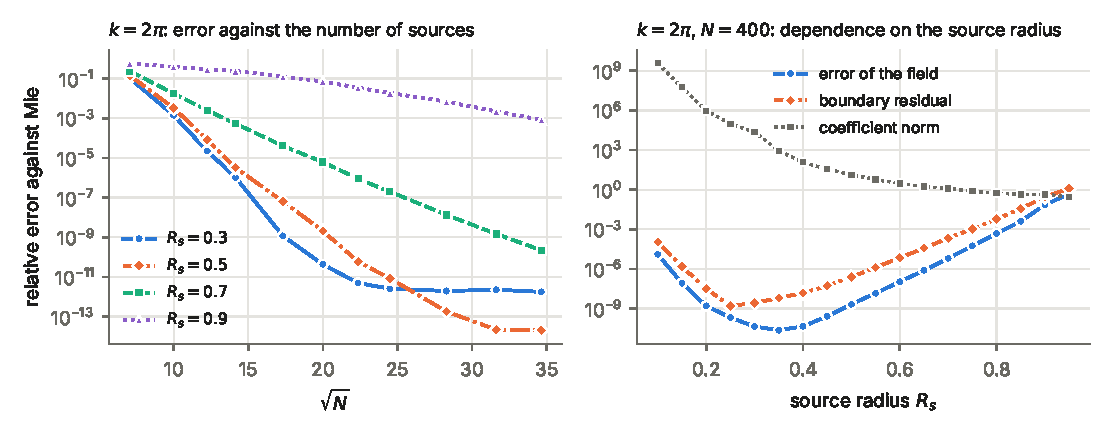
\includegraphics[width=0.95\textwidth]{fig_sphere_short.pdf}
  \caption{MFS for the perfectly conducting unit sphere at $k = 2\pi$, error against the Mie series. Left: error against $\sqrt{N}$ for four source radii $R$. Right: error, boundary residual and coefficient norm against $R$ for $N = 400$.}
  \label{fig:sphere}
\end{figure}

\subsection{The torus}
\label{sec:torus}

The sphere is forgiving because its only singularity is a point. Our second smooth body is the torus $(\rho - R)^2 + z^2 = a^2$, $\rho = \sqrt{x^2+y^2}$, with major radius $R = 1$ and minor radius $a = 0.5$, again at $k = 2\pi$. It is not convex and has no closed-form solution.

The sources are electric dipoles on an inner torus with the same centre circle and minor radius $a_s < a$, arranged on $n_s$ rings around the tube with $n_\varphi$ equally spaced dipoles per ring. The boundary points lie on $2n_s$ rings with $n_\varphi$ points each. Both sets are invariant under rotation by $2\pi/n_\varphi$ about the axis, so the least-squares problem splits exactly into $n_\varphi$ small problems, one for each Fourier mode about the axis, for any incident wave. This is the splitting used by Liu and Barnett for acoustic scattering \cite{liu2016}.

For the torus the admissible source surfaces are bounded from below. Let $c = \sqrt{R^2-a^2}$. The circle $\rho = c$, $z = 0$ is the focal ring of the toroidal coordinates in which the surface is a coordinate surface, and it lies inside the tube, between the centre circle and the inner wall. We find that the continued field is singular on the focal ring, so that a source torus concentric with the tube must satisfy
\begin{equation}
  a_s > R - \sqrt{R^2-a^2}.
  \label{eq:torusradius}
\end{equation}
We have not proved this bound and present it as a conjecture supported by an image argument and two numerical tests (\supp{3}). \autoref{fig:torussources} shows one of the tests. With a fixed number of sources, the norm of the coefficients stays of order one while $a_s$ satisfies \eqref{eq:torusradius} and grows by orders of magnitude below the bound, which is the behaviour that Barnett and Betcke prove for the disc \cite{barnett2008}. We know of no proof in the literature either. Millar's continuation theory for axially symmetric problems \cite{millar1983} assumes a body that meets the axis, and for tori in four and six dimensions the singular set of the related Schwarz potential is the centre circle alone \cite{aberra2002}.

\begin{figure}[htbp]
  \centering
  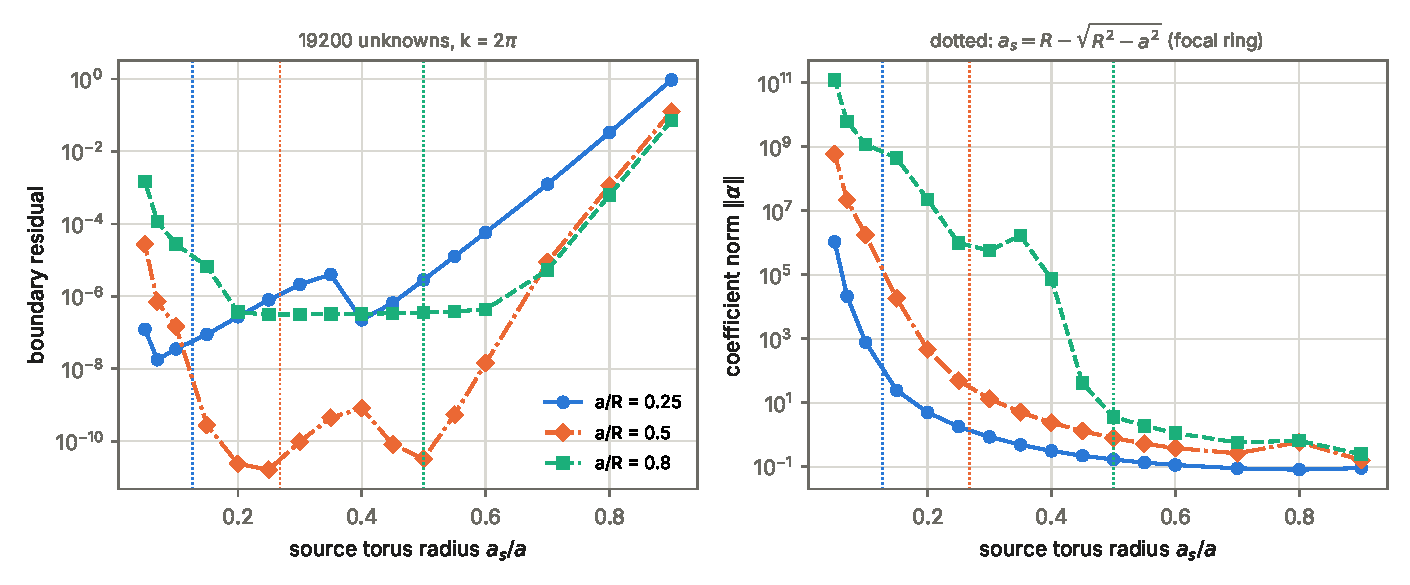
\includegraphics[width=0.85\textwidth]{fig_torus_sources.pdf}
  \caption{Torus with $R = 1$ and three minor radii $a$, $k = 2\pi$, $19200$ unknowns. Boundary residual (left) and coefficient norm (right) against the radius of the source torus. The dotted lines mark the bound \eqref{eq:torusradius}.}
  \label{fig:torussources}
\end{figure}

With $a_s = 0.5\,a$ the error of the scattered field, measured against the finest MFS run, falls from $5.0\times10^{-3}$ with $1440$ unknowns to $7.3\times10^{-12}$ with $21120$ unknowns, and the finest of these runs takes $10$\,s. As an independent check, the extinction cross-section computed by Bempp approaches the MFS value $11.7526$ like the reciprocal of the number of unknowns, and extrapolation gives $11.7533$, a relative difference of less than $10^{-4}$.
